\documentclass{ximera}

\newcommand{\RR}{\mathbb R}
\renewcommand{\d}{\,d}
\newcommand{\dd}[2][]{\frac{d #1}{d #2}}
\renewcommand{\l}{\ell}
\newcommand{\ddx}{\frac{d}{dx}}
\newcommand{\dfn}{\textbf}
\newcommand{\eval}[1]{\bigg[ #1 \bigg]}


\outcome{Recognize sequences as functions.}
\outcome{Graph sequences.}
\outcome{Use terminology for sequences.}
\outcome{Compute limits of sequences.}
\outcome{Understand growth rates of basic sequences.}
\outcome{Apply the monotone convergence theorem.}


\title[Dig-In:]{Sequences as functions}

\begin{document}
\begin{abstract}
A sequence can be thought of as a function from the integers to the real numbers.  There are two ways to establish whether a sequence has a limit.
\end{abstract}
\maketitle

Recall that in the previous section, we defined a sequence as an ordered list of numbers, and chose to adopt the notation $\{a_n\}_{n=1}$ to denote the list:

\[
a_1, a_2, a_3 , \ldots
\]

In the previous section, we studied different ways to generate the numbers in this list, special types of sequences, and new sequences that we could construct from a given one.  However, once we have a sequence, we can turn our attention to two fundamental questions regarding it:

\begin{itemize}
\item[1.] Do the numbers in the list approach a finite value?
\item[2.] Can I sum all of the numbers in the list?
\end{itemize}

We will address the first question in this section and the second question in the following section.  We begin by giving a definition:

%Jim's note: introducing the parallel here gives motivation to study limits...not entirely convinced this is a bad idea

\section{Limits of sequences}

Since sequences are essentially \dfn{discrete}, meaning that the points
are separate and distinct, the notion of a ``limit at a point'' cannot
be made to really make sense. However, limits at \textit{infinity} are
a different story.

In short, given a sequence, it is helpful to be able to say something
qualitative about it; we may want to address the question such as
``what happens after a while?'' 

Earlier, you've studied a similar question about
\[
\lim_{x\to\infty} f(x)
\]
when $x$ is a variable taking on real values; now, we simply want to
restrict the ``input'' values to be integers. No significant
difference is required in the definition of limit, except that we
specify, perhaps implicitly, that the variable is an integer:

\begin{definition}\index{limit of a sequence}
  Given a sequence $\{a_n\}_{n =n_0}$, we say that the \dfn{limit} of the sequence is $L$ if $a_n$ becomes arbitrarily close to $L$ as $n$ grows arbitrarily large.
  
If $\lim_{n\to\infty}a_n=L$ we say that the sequence
\dfn{converges}\index{convergent sequence}\index{sequence!convergent}.
If there is no finite value $L$ so that $\lim_{n\to\infty}a_n = L$,
then we say that the limit \dfn{does not exist}, or equivalently that
the sequence \dfn{diverges}\index{divergent
  sequence}\index{sequence!divergent}.
\end{definition}

\begin{question}
Suppose that $\{a_n\}_{n=1}$ is a sequence and that $\lim_{n \to \infty} = L$.  What can we say about $\lim_{n \to \infty} a_{n+1}$?
\begin{multipleChoice}
\choice{$\lim_{n \to \infty} a_{n+1}$ exists, but we do not know what its value is.}
\choice[correct]{$\lim_{n \to \infty} a_{n+1}$ exists, and $\lim_{n \to \infty} a_{n+1}=L$ exists.}
\choice{$\lim_{n \to \infty} a_{n+1}$ could exist but does not have to exist.}
\end{multipleChoice}

Note that the sequence $\{a_n\}_{n=1}$ is the list:

\[
a_1,a_2,a_3, \ldots
\]

while the sequence $\{a_{n+1}\}_{n=1}$ is:

\[
a_2,a_3,a_4, \ldots
\]

It should be clear that since the first sequences tends to $L$, the second sequence must also tend to $L$!
\end{question}


\begin{remark}
This definition of a limit can be made more precise as follows:

\begin{definition}\index{formal limit of a sequence}
\label{definition:limit-of-a-sequence}
Suppose that $\{a_n\}_{n=n_0}$ is a sequence.  We say that
$\lim_{n\to \infty}a_n=L$ if for every $\epsilon>0$, there exists an integer $N$, such that $|a_n-L|<\epsilon$ for any $n \geq N$.
\end{definition}

Here $\epsilon$ measures how close the terms in the sequence are to the limit $L$ and the above definition really states that no matter how close you want these terms to be, there is a value for the index $N$ so that \emph{all} subsequent terms in the sequence are at least that close to it!
\end{remark}




%\begin{question}
%  To say that the sequence $a_n$ converges to $L$ means what?  In
%  other words, what is the definition of the statement
%  $\lim_{n\to\infty} a_n = L$?
%  \begin{hint}
%    We are trying to make precise the idea that, eventually, all the elements of the sequence $a_n$ are as close as we want to $L$.
%  \end{hint}
%  \begin{hint}
%    To measure closeness to $L$, we will use a positive real number $\epsilon$.
%  \end{hint}
%  \begin{hint}
%    We must achieve any desired degree of closeness, so we will make a statement which is true for any positive real number $\epsilon$.
%  \end{hint}
%  \begin{hint}
%    In other words, the definition will begin ``For every positive real number $\epsilon > 0$\ldots''.
%  \end{hint}
%  \begin{hint}
%    We now must make precise the idea of ``eventually'' close.
%  \end{hint}
%  \begin{hint}
%    We use a whole number $N$ to capture the idea of ``sufficiently large'' values of $n$.
%  \end{hint}
%  \begin{hint}
%    Specifically, the definition will begin ``For every positive real number $\epsilon > 0$, there exists an $N \in \mathbb{N}$\ldots''
%  \end{hint}
%  \begin{hint}
%    The ``sufficiently large'' value of $n$ is any value which is at least as large as $N$.
%  \end{hint}
%  \begin{hint}
%    So, we will only consider those $n$ for which $n \ge N$.
%  \end{hint}
%    \begin{hint}
%      Thus the definition goes ``For every positive real number $\epsilon > 0$, there exists an $N \in \mathbb{N}$ so that whenever $n \ge N$\ldots''
%    \end{hint}
%    \begin{hint}
%      What happens ``eventually'' is that elements of the sequence are close to $L$.  How close?  Within $\epsilon$.
%    \end{hint}
%    \begin{hint}
%      The quantity $|a_n - L|$ is the distance between $a_n$ and $L$.
%    \end{hint}
%    \begin{hint}
%      To say that $a_n$ is within $\epsilon$ of $L$ is to say that $|a_n - L| < \epsilon$.
%    \end{hint}
%    \begin{hint}
%      Therefore the definition is ``For every positive real number $\epsilon > 0$ there exists an $N \in \mathbb{N}$ so that whenever $n \ge N$, we have $ |a_n - L| < \epsilon $.''
%    \end{hint}
%
%    \begin{multipleChoice}
%      \choice[correct]{For every positive real number $\epsilon > 0$ there exists an $N \in \mathbb{N}$ so that whenever $n \ge N$, we have $ |a_n - L| < \epsilon $.}
%      \choice{For every real number $\epsilon > 0$ there exists an $N \in \mathbb{N}$ so that $ |a_N - L| < \epsilon $.}
%      \choice{For every real number $\epsilon \in \mathbb{R}$ there exists an $N \in \mathbb{N}$ so that whenever $n \ge N$, we have $ |a_n - L| < \epsilon $.}
%      \choice{For every whole number $N > 0$ there exists a positive real number $\epsilon > 0$ so that whenever $n \ge N$, we have $ |a_n - L| < \epsilon $.}
%      \choice{For every whole number $N > 0$ there exists a real number $\epsilon \in \mathbb{R}$ so that whenever $n \ge N$, we have $ |a_n - L| < \epsilon $.}
%    \end{multipleChoice}
%    
%
%  The definition of limit can be written as if it were poetry with
%  line breaks and all.  Like the best of poems, it deserves to be
%  memorized, performed, and internalized.  Humanity struggled for millennia
%  to find the wisdom contained in this definition.
%\end{question}

\begin{warning}
  In the case that $\lim_{n \to \infty} a_n = \pm\infty$, we say that
  $\{a_n\}$ diverges.  \textbf{The only time we say that a sequence converges
    is when the limit exists and is equal to a \textit{finite} value}.
\end{warning}

%\youtube{https://www.youtube.com/watch?v=0UCRZAsIkXM}

We have previously studied how to compute limits, so the curious young mathematician could certainly ask whether the old techniques for continuous functions can still can be applied to find limits of sequences.

One way to compute the limit of a sequence is to compute the limit of
the related function.
\begin{theorem}
  Let $f(x)$ be a real-valued function.  If $a_n = f(n)$ defines a
  sequence and if
  \[
  \lim_{x\to\infty}f(x)=L,
  \]
  then $\lim_{n\to\infty} a_n=L$ as well.
\end{theorem}

\begin{warning}
It is important to note that the converse of this theorem is not
true. There are functions $f(x)$ and sequences $(a_n)$ where $a_n
=f(n)$ and
\[
\lim_{x\to\infty}f(x)=\text{DNE} \quad\text{but} \quad \lim_{n\to\infty} a_n = L
\]
for some number $L$.
\end{warning}

To show the converse is not true, it is enough to provide a single
example where it fails.  Here is such a counterexample.

\begin{example}
  Let $(a_n)$ be given by the rule $a_n = f(n)=\sin(n\pi)$. Show that
  \[
  \lim_{n\to\infty} a_n \ne \lim_{x\to \infty}f(x).
  \]
  \begin{explanation}
  The sequence $(a_n)$ is the sequence
  \[
  \sin(0\pi),\, \sin(1\pi),\, \sin(2\pi),\,\sin(3\pi),\,\ldots,
  \]
which is just the sequence $0, 0, 0, 0, \ldots$ since $\sin(n\pi)=0$
whenever $n$ is an integer.  Since the sequence is just the constant
sequence, we have
\[
\lim_{n\to\infty} f(n)= \lim_{n\to\infty} 0 = 0. 
\]
But $\lim_{x\to\infty}f(x)$, when $x$ is real, does not exist: as $x$
gets bigger and bigger, the values $\sin(x\pi)$ do not get closer and
closer to a single value, but instead oscillates between $-1$ and $1$.
  \end{explanation}
\end{example}

Here is some general advice. If you want to know $\lim_{n\to\infty}
a_n$, you might first think of a function $f(x)$ where $a_n = f(n)$,
and then attempt to compute $\lim_{x\to\infty}f(x)$.  If the limit of
the function exists, then it is equal to the limit of the sequence.
But, if for some reason $\lim_{x\to\infty}f(x)$ does not exist, it may
nevertheless still be the case that $\lim_{n\to\infty}a_n$ exists,
you'll just have to figure out another way to compute it.






%%%%%

Let's summarize the preceding section in the following formal definition.
\begin{definition}
  A \dfn{sequence} $(a_n)$ is a real-valued
  function with domain
  \[
  \{ n \in \Z : n \ge N \},\quad \text{for some integer $N$}
  \]
  where $\Z = \{\dots, -5,-4,-3,-2,-1,0,1,2,3,4,5,\dots,\}$ is the set
  of \dfn{integers}.\index{Z@$\Z$}
\end{definition}

Stated more humbly, a sequence assigns a real number to each of the integers
starting with an index $N$.

When thought of as a function, the ``outputs'' of a sequence are the
\dfn{elements} of the sequence; the ``$n$th element'' is the real
number that the sequence associates to the natural number $n$, and is
usually written $a_n$. \index{sequence!element} The $n$ in the phrase
``$n$th element'' is called an \dfn{index}\index{sequence!index}; the
plural of index is either indices or indexes, depending on who you
ask.  The first index $N$ is called the \dfn{initial index}.

\begin{question}
  What function corresponds to the sequence given by the explicit formula
  $a_n = -n/2+3$ for $n=1,2,3,\dots$?
  \begin{prompt}
    \[
    a(x) = \answer[given]{-x/2 + 3}
    \]
  \end{prompt}
\end{question}

\begin{question}
  What function corresponds to the sequence given by the explicit formula
  $a_n = 6\left(\frac{2}{5}\right)^{n+2}$ for $n=1,2,3,\dots$?
  \begin{prompt}
    \[
    a(x) = \answer[given]{6\left(\frac{2}{5}\right)^{x+2}}
    \]
  \end{prompt}
\end{question}

Since sequences can be conceptualized as functions, and calculus is
used to study functions, we can now apply our knowledge of calculus to
sequences!

\section{Plotting sequences}

First, we plot sequences as points. Later, we will see another
interpretation.

\subsection{Plots of arithmetic sequences}

Recall that arithmetic sequences are those where the difference
between neighboring elements is constant.  Arithmetic sequences are
analogues of lines.  Consider a basic example:
\begin{image}
  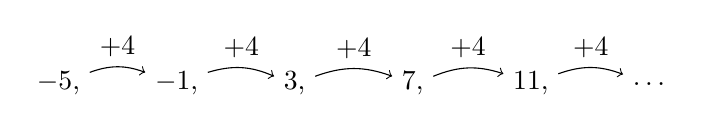
\begin{tikzpicture}[node distance=1.5cm]
    \node (a1) {$-5$,};
    \node (a2) [right of=a1] {$-1$,};
    \node (a3) [right of=a2] {$3$,};
    \node (a4) [right of=a3] {$7$,};
    \node (a5) [right of=a4] {$11$,};
    \node (a6) [right of=a5] {$\ldots$};
    
    \path[->] (a1) edge [bend left=20] node[above]{$+4$} (a2);
    \path[->] (a2) edge [bend left=20] node[above]{$+4$} (a3);
    \path[->] (a3) edge [bend left=20] node[above]{$+4$} (a4);
    \path[->] (a4) edge [bend left=20] node[above]{$+4$} (a5);
    \path[->] (a5) edge [bend left=20] node[above]{$+4$} (a6);
  \end{tikzpicture}
\end{image}

Check out a graph of the sequence:

\begin{image}
\begin{tikzpicture}
	\begin{axis}[
            domain=0:6,xmin=0,xmax=6,ymin=-9,ymax=15,
            width=4in,
            height=2in,
            axis lines =middle, xlabel=$n$, ylabel=$a$,
            xtick={1,2,...,5},
            ytick={-5,-1,...,11},
            yticklabels={$a_1 = -5$,$a_2=-1$,$a_3=3$,$a_4=7$,$a_5=11$},
            every axis y label/.style={at=(current axis.above origin),anchor=south},
            every axis x label/.style={at=(current axis.right of origin),anchor=west},
            clip=false,
            %axis on top,
          ]
          \addplot[color=penColor,fill=penColor,only marks,mark=*] coordinates{(1,-5)};  %% closed hole          
          \addplot[color=penColor,fill=penColor,only marks,mark=*] coordinates{(2,-1)};  %% closed hole          
          \addplot[color=penColor,fill=penColor,only marks,mark=*] coordinates{(3,3)};  %% closed hole          
          \addplot[color=penColor,fill=penColor,only marks,mark=*] coordinates{(4,7)};  %% closed hole          
          \addplot[color=penColor,fill=penColor,only marks,mark=*] coordinates{(5,11)};  %% closed hole  
        \end{axis}
\end{tikzpicture}
\end{image}

Here is an arithmetic sequence that decreases as its index increases.

\begin{image}
  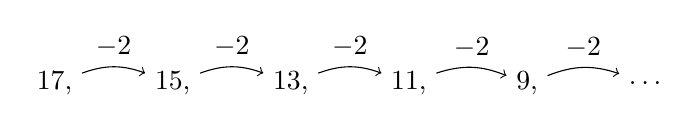
\begin{tikzpicture}[node distance=1.5cm]
    \node (a1) {$17$,};
    \node (a2) [right of=a1] {$15$,};
    \node (a3) [right of=a2] {$13$,};
    \node (a4) [right of=a3] {$11$,};
    \node (a5) [right of=a4] {$9$,};
    \node (a6) [right of=a5] {$\ldots$};

    \path[->] (a1) edge [bend left=20] node[above]{$-2$} (a2);
    \path[->] (a2) edge [bend left=20] node[above]{$-2$} (a3);
    \path[->] (a3) edge [bend left=20] node[above]{$-2$} (a4);
    \path[->] (a4) edge [bend left=20] node[above]{$-2$} (a5);
    \path[->] (a5) edge [bend left=20] node[above]{$-2$} (a6);
  \end{tikzpicture}
\end{image}

Here we see a graph:

\begin{image}
\begin{tikzpicture}
	\begin{axis}[
            domain=0:6,xmin=0,xmax=6,ymin=7,ymax=19,
            width=4in,
            height=2in,
            xtick={1,2,...,5},
            ytick={17,15,...,9},
            yticklabels={$a_1 = 17$,$a_2=15$,$a_3=13$,$a_4=11$,$a_5=9$},
            axis lines =middle, xlabel=$n$, ylabel=$a$,
            every axis y label/.style={at=(current axis.above origin),anchor=south},
            every axis x label/.style={at=(current axis.right of origin),anchor=west},
            clip=false,
            %axis on top,
          ]
          \addplot[color=penColor,fill=penColor,only marks,mark=*] coordinates{(1,17)};  %% closed hole          
          \addplot[color=penColor,fill=penColor,only marks,mark=*] coordinates{(2,15)};  %% closed hole          
          \addplot[color=penColor,fill=penColor,only marks,mark=*] coordinates{(3,13)};  %% closed hole          
          \addplot[color=penColor,fill=penColor,only marks,mark=*] coordinates{(4,11)};  %% closed hole          
          \addplot[color=penColor,fill=penColor,only marks,mark=*] coordinates{(5,9)};  %% closed hole  
        \end{axis}
\end{tikzpicture}
\end{image}


\begin{question}
  To what type of curve do arithmetic sequences correspond?
  \begin{multipleChoice}
    \choice[correct]{lines}
    \choice{parabolas}
    \choice{polynomials}
    \choice{exponential curves}
    \choice{impossible to say}
  \end{multipleChoice}
  \begin{feedback}
    Since the average growth rate of a line is constant regardless of
    the size of the interval chosen, arithmetic sequences correspond to
    lines.
  \end{feedback}
\end{question}


\subsection{Plots of geometric sequences}

Recall that geometric sequences are those where the ratio between
neighboring elements is constant.  When this ratio is positive, a
geometric sequence corresponds to an exponential function. Consider a
basic example:
\begin{image}
    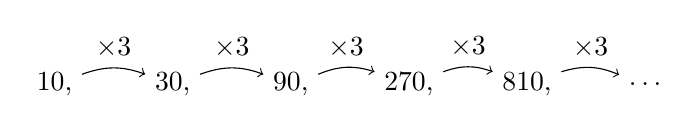
\begin{tikzpicture}[node distance=1.5cm]
    \node (a1) {$10$,};
    \node (a2) [right of=a1] {$30$,};
    \node (a3) [right of=a2] {$90$,};
    \node (a4) [right of=a3] {$270$,};
    \node (a5) [right of=a4] {$810$,};
    \node (a6) [right of=a5] {$\ldots$};

    \path[->] (a1) edge [bend left=20] node[above] {$\times 3$} (a2);
    \path[->] (a2) edge [bend left=20] node[above] {$\times 3$} (a3);
    \path[->] (a3) edge [bend left=20] node[above] {$\times 3$} (a4);
    \path[->] (a4) edge [bend left=20] node[above] {$\times 3$} (a5);
    \path[->] (a5) edge [bend left=20] node[above] {$\times 3$} (a6);
  \end{tikzpicture}
\end{image}
Let's see a graph: 
\begin{image}
\begin{tikzpicture}
	\begin{axis}[
            domain=0:6,xmin=0,xmax=6,ymin=-100,ymax=900,
            width=4in,
            height=2in,
            xtick={1,2,...,5},
            ytick={10,30,90,270,810},
            yticklabels={},%$a_1 = 10$,$a_2=30$,$a_3=90$,$a_4=270$,$a_5=810$},
            axis lines =middle, xlabel=$n$, ylabel=$a$,
            every axis y label/.style={at=(current axis.above origin),anchor=south},
            every axis x label/.style={at=(current axis.right of origin),anchor=west},
            clip=false,
            %axis on top,
          ]
          \addplot[color=penColor,fill=penColor,only marks,mark=*] coordinates{(1,10)};  %% closed hole          
          \addplot[color=penColor,fill=penColor,only marks,mark=*] coordinates{(2,30)};  %% closed hole          
          \addplot[color=penColor,fill=penColor,only marks,mark=*] coordinates{(3,90)};  %% closed hole          
          \addplot[color=penColor,fill=penColor,only marks,mark=*] coordinates{(4,270)};  %% closed hole          
          \addplot[color=penColor,fill=penColor,only marks,mark=*] coordinates{(5,810)};  %% closed hole  
        \end{axis}
\end{tikzpicture}
\end{image}

If the common ratio of a geometric sequence is between $0$ and $1$, a
geometric sequence will decrease as it progresses.

\begin{image}
  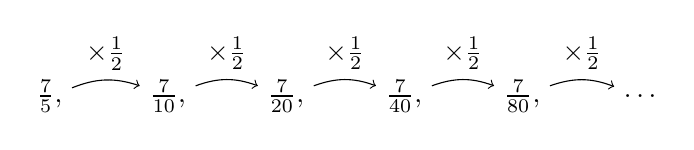
\begin{tikzpicture}[node distance=1.5cm]
    \node (a1) {$\frac{7}{5}$,};
    \node (a2) [right of=a1] {$\frac{7}{10}$,};
    \node (a3) [right of=a2] {$\frac{7}{20}$,};
    \node (a4) [right of=a3] {$\frac{7}{40}$,};
    \node (a5) [right of=a4] {$\frac{7}{80}$,};
    \node (a6) [right of=a5] {$\ldots$};
    
    \path[->] (a1) edge [bend left=20] node[above] {$\times\frac{1}{2}$} (a2);
    \path[->] (a2) edge [bend left=20] node[above] {$\times\frac{1}{2}$} (a3);
    \path[->] (a3) edge [bend left=20] node[above] {$\times\frac{1}{2}$} (a4);
    \path[->] (a4) edge [bend left=20] node[above] {$\times\frac{1}{2}$} (a5);
    \path[->] (a5) edge [bend left=20] node[above] {$\times\frac{1}{2}$} (a6);
  \end{tikzpicture}
\end{image}
Let's see a graph:
\begin{image}
\begin{tikzpicture}
	\begin{axis}[
            domain=0:6,xmin=0,xmax=6,ymin=0,ymax=2,
            width=4in,
            height=2in,
            xtick={1,2,...,5},
            ytick={1.4,.7,.35,.175,.0875},
            yticklabels={},%$a_1 = 10$,$a_2=30$,$a_3=90$,$a_4=270$,$a_5=810$},
            axis lines =middle, xlabel=$n$, ylabel=$a$,
            every axis y label/.style={at=(current axis.above origin),anchor=south},
            every axis x label/.style={at=(current axis.right of origin),anchor=west},
            clip=false,
            %axis on top,
          ]
          \addplot[color=penColor,fill=penColor,only marks,mark=*] coordinates{(1,7/5)};  %% closed hole          
          \addplot[color=penColor,fill=penColor,only marks,mark=*] coordinates{(2,7/10)};  %% closed hole          
          \addplot[color=penColor,fill=penColor,only marks,mark=*] coordinates{(3,7/20)};  %% closed hole          
          \addplot[color=penColor,fill=penColor,only marks,mark=*] coordinates{(4,7/40)};  %% closed hole          
          \addplot[color=penColor,fill=penColor,only marks,mark=*] coordinates{(5,7/80)};  %% closed hole  
        \end{axis}
\end{tikzpicture}
\end{image}


\begin{question}
  When the common ratio between successive elements of a geometric sequence is positive, what
  type of curves do geometric sequences correspond to?
  \begin{multipleChoice}
    \choice{lines}
    \choice{parabolas}
    \choice{polynomials}
    \choice[correct]{exponential curves}
    \choice{impossible to say}
  \end{multipleChoice}
  \begin{feedback}
  If a geometric sequence is expressed as $a_n = a_1 \cdot r^{n-1}$,
  then in function notation we have $a(x) = a_1 \cdot r^{x-1}$, an
  exponential function.
  \end{feedback}
\end{question}



On the other hand, if the common ration between successive elements of
a geometric sequence is \textbf{not} positive, then something
interesting happens. Check out this example:
\begin{image}
  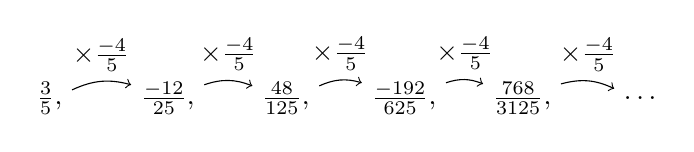
\begin{tikzpicture}[node distance=1.5cm]
    \node (a1) {$\frac{3}{5}$,};
    \node (a2) [right of=a1] {$\frac{-12}{25}$,};
    \node (a3) [right of=a2] {$\frac{48}{125}$,};
    \node (a4) [right of=a3] {$\frac{-192}{625}$,};L
    \node (a5) [right of=a4] {$\frac{768}{3125}$,};
    \node (a6) [right of=a5] {$\ldots$};
    
    \path[->] (a1) edge [bend left=20] node[above] {$\times\frac{-4}{5}$} (a2);
    \path[->] (a2) edge [bend left=20] node[above] {$\times\frac{-4}{5}$} (a3);
    \path[->] (a3) edge [bend left=20] node[above] {$\times\frac{-4}{5}$} (a4);
    \path[->] (a4) edge [bend left=20] node[above] {$\times\frac{-4}{5}$} (a5);
    \path[->] (a5) edge [bend left=20] node[above] {$\times\frac{-4}{5}$} (a6);
  \end{tikzpicture}
\end{image}
Let's see a graph:
\begin{image}
\begin{tikzpicture}
	\begin{axis}[
            domain=0:6,xmin=0,xmax=6,ymin=-.7,ymax=.7,
            width=4in,
            height=2in,
            xtick={1,2,...,5},
            ytick={.6,-.48,.384,-.3072,.24576},
            yticklabels={},%$a_1 = 10$,$a_2=30$,$a_3=90$,$a_4=270$,$a_5=810$},
            axis lines =middle, xlabel=$n$, ylabel=$a$,
            every axis y label/.style={at=(current axis.above origin),anchor=south},
            every axis x label/.style={at=(current axis.right of origin),anchor=west},
            clip=false,
            %axis on top,
          ]
          \addplot[color=penColor,fill=penColor,only marks,mark=*] coordinates{(1,3/5)};  %% closed hole          
          \addplot[color=penColor,fill=penColor,only marks,mark=*] coordinates{(2,-12/25)};  %% closed hole          
          \addplot[color=penColor,fill=penColor,only marks,mark=*] coordinates{(3,48/125)};  %% closed hole          
          \addplot[color=penColor,fill=penColor,only marks,mark=*] coordinates{(4,-192/625)};  %% closed hole          
          \addplot[color=penColor,fill=penColor,only marks,mark=*] coordinates{(5,768/3125)};  %% closed hole  
        \end{axis}
\end{tikzpicture}
\end{image}
The sign of this sequence alternates! 

\subsection{Monotonicity}

We'd like some terminology to describe features we might
notice about sequences.  Here is some of that terminology, focused on the relationships between the terms of a sequence.

\begin{definition}
  A sequence is called
  \begin{itemize}
    \item \dfn{increasing} if $a_n<a_{n+1}$ for all $n$,
    \item \dfn{nondecreasing} if $a_n\le a_{n+1}$ for all $n$,
    \item \dfn{decreasing} if $a_n>a_{n+1}$ for all $n$,
    \item \dfn{nonincreasing} if $a_n\ge a_{n+1}$ for all $n$.
  \end{itemize}
\end{definition}

Lots of facts are true for sequences which are either increasing or
decreasing; to talk about this situation without constantly saying
``either increasing or decreasing,'' we can make up a single word to
cover both cases.
\begin{definition}
  If a sequence is
  \begin{itemize}
  \item increasing, or
  \item nondecreasing, or
  \item decreasing, or
  \item nonincreasing,
  \end{itemize}
  it is said to be \dfn{monotonic}\index{sequence!monotonic}.
\end{definition}

\begin{question}
  If an arithmetic sequence $a_n = m\cdot n + b$ is monotonic, what
  must be true about $m$ and $b$?
  \begin{prompt}
    \begin{quote}
      The sign of $m$ \wordChoice{\choice{is positive}\choice{is
          negative}\choice[correct]{does not matter}}, and the sign of $b$ is
      \wordChoice{\choice{is positive}\choice{is negative}\choice[correct]{does
          not matter}}
    \end{quote}
  \end{prompt}
  \begin{feedback}
    An arithmetic sequence is always monotonic, regardless of the
    values of $m$ and $b$.
  \end{feedback}
\end{question}

\begin{question}
  If a geometric sequence $a_n = a_1 \cdot r^{n-1}$ is monotonic, what
  must be true about $a_1$ and $r$?
  \begin{prompt}
    \begin{quote}
      The sign of $a_1$ \wordChoice{\choice{is positive}\choice{is
          negative}\choice[correct]{does not matter}}, and the sign of
      $r$ is \wordChoice{\choice[correct]{is positive}\choice{is
          negative}\choice{does not matter}}
    \end{quote}
  \end{prompt}
    \begin{feedback}
    A geometric sequence $a_n = a_1 \cdot r^{n-1}$ is monotonic if and
    only if the sign of $r$ is positive.
  \end{feedback}
\end{question}

Let's see some examples:
\begin{example}
  Describe the growth of $a_n = \frac{2^n-1}{2^n}$ for
  $n=1,2,3,\dots$.
  \begin{explanation}
    To do this, check out the difference between two sequential terms,
    write with me:
    \begin{align*}
    a_{n+1} - a_n &= \answer[given]{\frac{2^{n+1}-1}{2^{n+1}}} - \frac{2^n-1}{2^n}\\
    &=\frac{2^{n+1}-1 - 2\left(\answer[given]{2^n-1}\right)}{2^{n+1}}\\
    &=\frac{2^{n+1}-1 - 2^{n+1}+2}{2^{n+1}}\\
    &=\frac{\answer[given]{1}}{2^{n+1}}.
    \end{align*}
    Since $\frac{1}{2^{n+1}}$ is always
    \wordChoice{\choice[correct]{positive}\choice{negative}\choice{zero}},
    we see that $(a_n)$ is
    \wordChoice{\choice[correct]{increasing}\choice{nondecreasing}\choice{decreasing}\choice{nonincreasing}}, and hence is \wordChoice{\choice[correct]{monotonic}\choice{not monotonic}}.
  \end{explanation}
\end{example}

\begin{example}
  Describe the growth of $a_n = \frac{n+1}{n}$ for $n=1,2,3,\dots$.
  \begin{explanation}
    To do this, check out the difference between two sequential terms.
    Write with me.
    \begin{align*}
    a_{n+1} - a_n &= \answer[given]{\frac{(n+1)+1}{n+1}} - \frac{n+1}{n}\\
    &=\frac{n(n+2) - (n+1)(\answer[given]{n+1})}{n+1}\\
    &=\frac{n^2+2n - n^2 -2n-1}{n+1}\\
    &=\frac{\answer[given]{-1}}{n+1}.
    \end{align*}
    Since $\frac{-1}{n+1}$ is always
    \wordChoice{\choice{positive}\choice[correct]{negative}\choice{zero}} for the values of $n$ we are considering,
    we see that $(a_n)$ is
    \wordChoice{\choice{increasing}\choice{nondecreasing}\choice[correct]{decreasing}\choice{nonincreasing}}, and hence is \wordChoice{\choice[correct]{monotonic}\choice{not monotonic}}.
  \end{explanation}
\end{example}

Sometimes we can say that the sequence doesn't get too big or too
small, in this case we say the sequence is \textit{bounded}.

\begin{definition}
  \label{definition:sequence-bounded}
  A sequence $(a_n)$ is \dfn{bounded} if there is some number $M$ so
  that for all $n$, we have $|a_n|\le M$.
\end{definition}

\begin{question}
  True or False: If a sequence $(a_n)_{n=0}^\infty$ is nondecreasing
  it is bounded below by $a_0$.
  \begin{prompt}
    \begin{multipleChoice}
    \choice[correct]{true}
    \choice{false}
    \end{multipleChoice}
  \end{prompt}
  \begin{feedback}
    If a sequence is nondecreasing, then its smallest value is its
    first element.
  \end{feedback}
\end{question}


\begin{question}
  True or False: If a sequence $(a_n)_{n=0}^\infty$ is nonincreasing
  it is bounded above by $a_0$.
  \begin{prompt}
    \begin{multipleChoice}
    \choice[correct]{true}
    \choice{false}
    \end{multipleChoice}
  \end{prompt}
  \begin{feedback}
    If a sequence is nonincreasing, then its largest value is its
    first element.
  \end{feedback}
\end{question}




\section{Monotone convergence}

We can now state an important theorem.

\begin{theorem}[Bounded-monotone convergence]
  If the sequence $a_n$ is bounded and monotonic, then
  \[
  \lim_{n \to  \infty} a_n = L
  \]
  for some real-number $L$.
\end{theorem}
\begin{question}
  Consider the sequence $a_{n}$.  Suppose you know that for all $n >
  1$,
  \[
  -6 \le a_{n} \le 0
  \]
  and $a_{1} = 2$, and $a_{2} = -1$, and that the sequence is
  nonincreasing.  Does the sequence converge?
  \begin{hint}
    Since the sequence is nonincreasing, the sequence is monotone.
  \end{hint}
  \begin{hint}
    Since for all $n \ge 1$, we have $a_{n} \ge -6$, the sequence is
    bounded below.
  \end{hint}
  \begin{hint}
    So by the Monotone Convergence Theorem, the sequence converges to
    some value; let us call it $L$.
  \end{hint}
  \begin{hint}
    Now consider the direction in which the sequence is heading.
  \end{hint}
  \begin{hint}
    Since the sequence is nonincreasing, for all $n \ge 2$, we have
    $-6 \le a_{n} \le -1$.
  \end{hint}
  \begin{hint}
    The limit $L$ must be in that interval as well.
  \end{hint}
  \begin{hint}
    Therefore the sequence converges to a value $L$ so that $-6 \le L
    \le -1$.
  \end{hint}
  \begin{prompt}
  \begin{multipleChoice}
    \choice[correct]{Yes, with limit between $-6$ and $-1$.}
    \choice{No, the sequence does not converge.}
    \choice{Yes, with limit between $-1$ and $0$.}
  \end{multipleChoice}
  \end{prompt}
\end{question}

In short, bounded monotonic sequences always converge, though we can't
necessarily describe the number to which they converge.  Let's try
some examples!

\begin{example}
  Given the sequence $a_n=\frac{2^n-1}{2^n}$ for $n=1,2,3,\dots$,
  explain how you know that $\lim_{n\to\infty} a_n$ converges to a
  finite value.
  \begin{explanation}
    To start, from previous work we know that $a_n$ is
    \wordChoice{\choice[correct]{monotonic}\choice{not monotonic}}.
    Moreover, all of the elements $a_n = (2^n-1)/2^n$ are less than
    $2$, and greater than zero. Hence by the bounded-monotone
    convergence theorem, $\lim_{n\to\infty} a_n$ converges to a finite
    value.
  \end{explanation}
\end{example}

\begin{example}
  Given the sequence $a_n=\frac{n+1}{n}$ for $n=1,2,3,\dots$,
  explain how you know that $\lim_{n\to\infty} a_n$ converges to a
  finite value.
  \begin{explanation}
    To start, from previous work we know that $a_n$ is
    \wordChoice{\choice[correct]{monotonic}\choice{not monotonic}}.
    Moreover, all of the elements $a_n = (n+1)/n$ are less than $2$,
    and greater than zero. Hence by the bounded-monotone convergence
    theorem, $\lim_{n\to\infty} a_n$ converges to a finite value.
  \end{explanation}
\end{example}

We don't actually need to know that a sequence is monotonic to apply
the bounded-monotone convergence theorem. It is enough to know that
the sequence is ``eventually'' monotonic, that is, that some point it
becomes increasing or decreasing.

\begin{example}
Show that the sequence $(a_n)$ given by $a_n = n^{1/n}$ converges.
\begin{explanation}
  We might first show that this sequence is decreasing, that is, we show
  that for all $n$,
  \[
  n^{1/n} > (n+1)^{1/(n+1)}.
  \]
  But this isn't true!  Take a look
  \begin{align*}
    a_1 &= 1, \\
    a_2 &= \sqrt{2} \approx 1.4142, \\
    a_3 &= \sqrt[3]{3} \approx 1.4422, \\
    a_4 &= \sqrt[4]{4} \approx 1.4142, \\
    a_5 &= \sqrt[5]{5} \approx 1.3797, \\
    a_6 &= \sqrt[6]{6} \approx 1.3480, \\
    a_7 &= \sqrt[7]{7} \approx 1.3205, \\
    a_8 &= \sqrt[8]{8} \approx 1.2968, \\
    a_9 &= \sqrt[9]{9} \approx 1.2765.
  \end{align*}
  But it does seem that this sequence perhaps is decreasing after the
  first few terms.  Can we justify this?

  Yes!  Consider the real function $f(x)=x^{1/x}$ when $x\ge 1$.  We
  compute the derivative, perhaps via \index{logarithmic
    differentiation}logarithmic differentiation, to find
  \[
  f'(x)=\answer[given]{\frac{x^{1/x} (1-\ln(x))}{x^2}}.
  \]
  Note that when $x\ge 3$, the derivative $f'(x)$ is negative.  Since
  the function $f$ is decreasing, we can conclude that the sequence is
  decreasing---well, at least for $n \geq 3$.

  Since all terms of the sequence are positive, the sequence is
  decreasing and bounded $0\le a_n \le a_3$ when $n \ge 3$, and so the
  sequence converges.
\end{explanation}
\end{example}



\subsection{The squeeze theorem}

Previously, when considering limits, one of our techniques was to replace 
complicated functions by simpler functions. The \textit{Squeeze Theorem}
tells us one situation where this is possible.

\begin{theorem}[Squeeze Theorem]\index{Squeeze Theorem}
  Suppose that $(a_n)$, $(b_n)$, and $(c_n)$ are sequences with
  \[
  a_n \le b_n \le c_n
  \]
  for all $n$ greater than some index $N$. If
  \[
  \lim_{n\to\infty} a_n = L = \lim_{n\to\infty} c_n,
  \] 
  then $\lim_{n\to\infty} b_n = L$.
\end{theorem}

Let's see an example.

\begin{example}
  Consider the sequence $(b_n)_{n=1}^{\infty}$ where $b_n =
  \left(\frac{-1}{2}\right)^n$. Compute:
  \[
  \lim_{n\to\infty}b_n
  \]
  \begin{explanation}
    To compute this limit we will use the squeeze theorem. Write with
    me:
    \[
    -\left(\frac{1}{2}\right)^n\le \left(\frac{-1}{2}\right)^n \le \left(\frac{1}{2}\right)^n
    \]
    but we know
    \[
    \lim_{n\to \infty}\left(-\left(\frac{1}{2}\right)^n\right) = \answer[given]{0}
    \]
    and
    \[
    \lim_{n\to \infty}\left(\frac{1}{2}\right)^n =\answer[given]{0}.
    \]
    Hence by the squeeze theorem, $\lim_{n\to\infty} b_n = \answer[given]{0}$.
  \end{explanation}
\end{example}


This last result actually gives us a general theorem about geometric
sequences:

\begin{theorem}
  Given a geometric sequence $a_n = a_1 \cdot r^{n-1}$,
  \[
  \lim_{n\to\infty} a_n =
  \begin{cases}
    0 &\text{if $|r|<1$,}\\
    1 &\text{if $r=1$,}\\
    \text{DNE} &\text{if $|r|>1$ or $r=-1$.}
  \end{cases}
  \]
\end{theorem}


\section{Growth rates}

When dealing with functions of real numbers, derivatives tell us the
instantaneous growth rate of a function. Since sequences are essentially
discrete, derivatives cannot really be used. Nevertheless, the idea of
a growth rate is still very important.

\begin{definition}
  Given two sequences $(a_n)$ and $(b_n)$, the notation $(a_n) \ll
  (b_n)$ means that
  \[
  \lim_{n\to\infty} \frac{a_n}{b_n} =
  0\qquad\text{and}\qquad\lim_{n\to\infty} \frac{b_n}{a_n} =\infty.
  \]
\end{definition}

In essence, writing $a_n \ll b_n$ says that the sequence $(b_n)$ grows
much faster than $(a_n)$.


\begin{theorem}[Growth rates of sequences]
  Let $p,q$ be positive real numbers, and let $b> 1$. We have the
  following relationship:
  \[
  (\ln^p(n))\ll (n^q) \ll (b^n) \ll (n!) \ll (n^n)
  \]
\end{theorem}

\begin{example}
  Let $a_n  = \frac{n^3\ln^{9}(n)}{n^4}$. Compute:
  \[
  \lim_{n\to \infty}a_n
  \]
  \begin{explanation}
    Let's simplify this a bit, write with me:
    \begin{align*}
      a_n &= \frac{n^3\ln^{9}(n)}{n^4}\\
      &= \frac{\ln^{9}(n)}{\answer[given]{n}}.
    \end{align*}
    Since
    \[
    (\ln^{9}(n))\ll (n)
    \]
    we see that $\lim_{n\to\infty}a_n =\answer[given]{0}$.  In short, the 
    denominator ``wins out'' over the numerator, so the terms of the 
    sequence get closer to zero.
  \end{explanation}
\end{example}


\end{document}
